% !TeX root = simplesnt-doc.tex
\documentclass{simplesnt}

%% Helpful packages
\usepackage{simplebnf}[2023/11/25]
\usepackage{kotex}
\usepackage{xcolor}
\usepackage{amsmath,amssymb}
\usepackage{amsfonts}
\usepackage{tikz}
\usetikzlibrary{calc}
\usepackage{siunitx}
\usepackage{caption}
\usepackage{listings}
\usepackage{mathrsfs}
\usepackage{stmaryrd}
\usepackage{subcaption}
\usepackage{graphicx}


\captionsetup{font=small}
\lstset{basicstyle = \small\ttfamily, breaklines}

\usepackage{tabularray}
\UseTblrLibrary{booktabs}

\usepackage{metalogo}
\usepackage{kotex-logo}


\newcommand{\textalt}[2]{#1\textsubscript{\ensuremath{\text{\scriptsize\textit{#2}}}}}
\newcommand*{\presentfont}[1]{{\fontspec{#1}#1}}
\ExplSyntaxOn
\bool_if:nF { \sys_if_engine_xetex_p: || \sys_if_engine_luatex_p: }
  { \newcommand*{\fontspec}[1]{} }
\ExplSyntaxOff

\title{정적 분석 골탕먹이기 논문 리뷰}
\author{정원준}

\begin{document}
\date{2026년 3월 6일}
\maketitle


\begin{frame}
  \frametitle{목차}
  \tableofcontents
\end{frame}


\begin{frame}
  \frametitle{슬라이드 제목}
  결론 대뜸 박기 할까말까
\end{frame}

\section{논문 소개}
\begin{frame}
  \frametitle{제목}
  
  \vspace{38pt}

  
\includegraphics[
    width=1\linewidth
  ]{img/제목.png}

  \begin{tikzpicture}[overlay, remember picture]
    \uncover<1>{
        \fill[white] (0,0) rectangle (12,1.3);
        \fill[white] (0,0) rectangle (1.8,2);
    }
    \uncover<2>{
        \fill[white] (0,0) rectangle (12,1.3);
    }
    \uncover<3>{
    }
  \end{tikzpicture}

  \vspace{-20pt}

  \begin{align*}
    \uncover<1->{P_1 \approx P_2 &\overset{\mathrm{def}}{\iff} \llbracket P_1 \rrbracket = \llbracket P_2 \rrbracket}  \\
    \uncover<2->{P_1 \approx^{\mathcal{A}} P_2 &\overset{\mathrm{def}}{\iff} \llbracket P_1 \rrbracket^{\mathcal{A}} = \llbracket P_2 \rrbracket^{\mathcal{A}}} \\
  \end{align*}

\end{frame}


\section{배경}
\begin{frame}
  \frametitle{의미구조}
  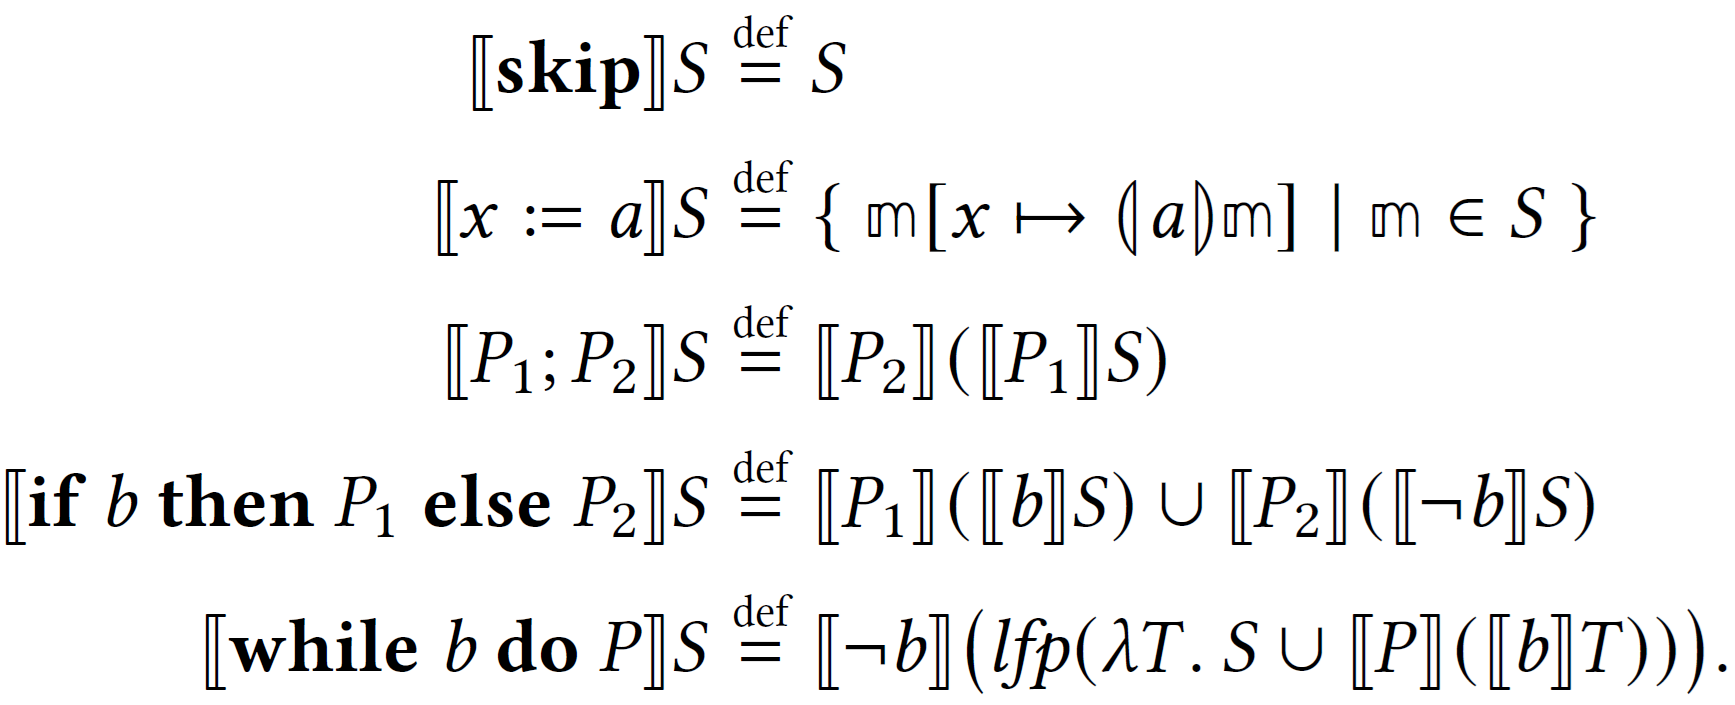
\includegraphics[scale=0.24]{img/의미구조.png}
\end{frame}

\begin{frame}
  \frametitle{요약의미구조}
  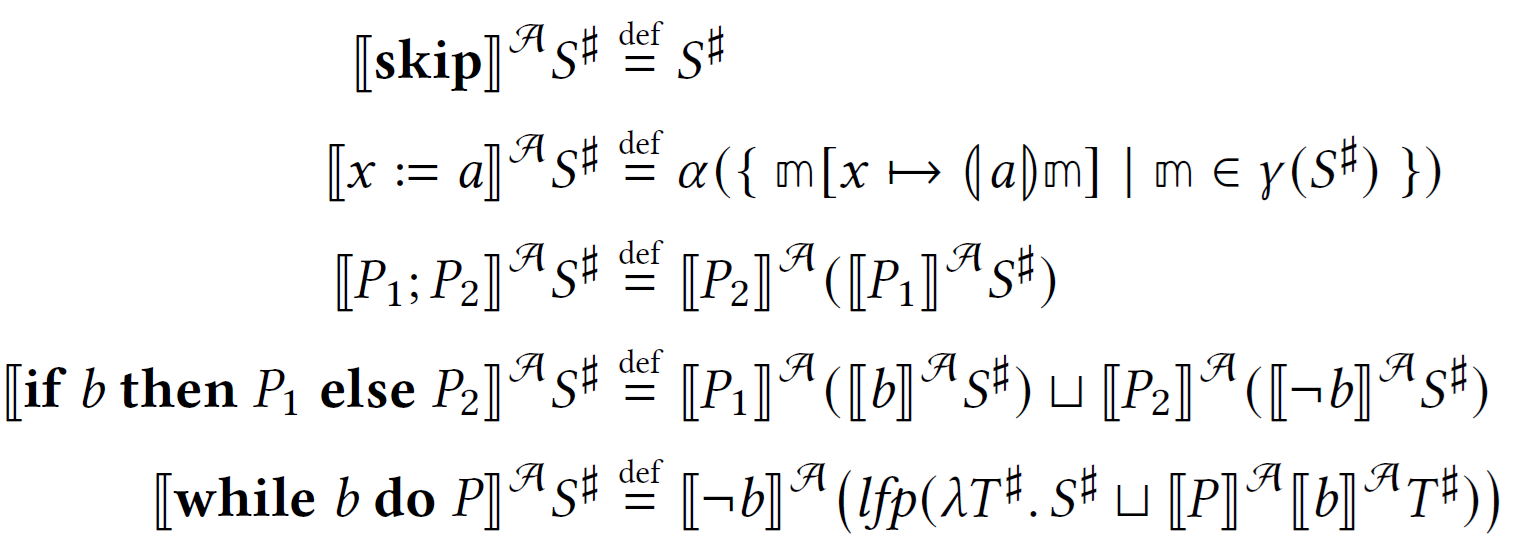
\includegraphics[scale=0.3]{img/요약의미구조.png}
\end{frame}

\begin{frame}
  \frametitle{가정}
  \uncover<1->{1. Galois insertion}
  \begin{figure}[h]
    \centering
    \begin{subfigure}{0.45\textwidth}
        \centering
        \uncover<2->{
          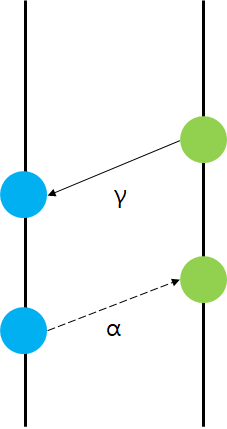
\includegraphics[width=\linewidth,height=0.75\textheight,keepaspectratio]{img/갈루아커넥션1.png}
        }
    \end{subfigure}
    \hfill
    \begin{subfigure}{0.45\textwidth}
        \centering
        \uncover<3->{
          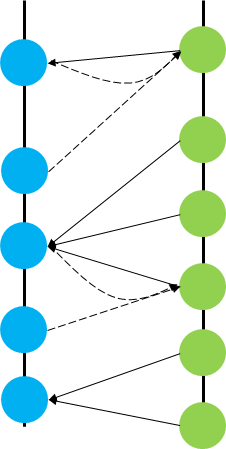
\includegraphics[width=\linewidth,height=0.75\textheight,keepaspectratio]{img/갈루아커넥션2.png}
        }
    \end{subfigure}
  \end{figure}
\end{frame}

\begin{frame}
  \frametitle{가정}
  \uncover<1->{1. Galois insertion}
  \begin{figure}[h]
    \centering
    \begin{subfigure}{0.45\textwidth}
        \centering
        \uncover<2->{
          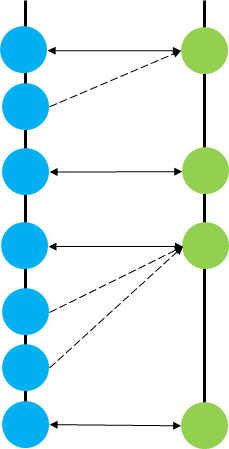
\includegraphics[width=\linewidth,height=0.75\textheight,keepaspectratio]{img/갈루아인서션1.png}
        }
    \end{subfigure}
    \hfill
    \begin{subfigure}{0.45\textwidth}
        \centering
        \uncover<3->{
          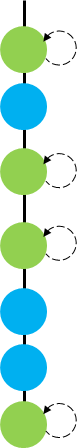
\includegraphics[width=\linewidth,height=0.75\textheight,keepaspectratio]{img/갈루아인서션2.png}
        }
    \end{subfigure}
  \end{figure}
\end{frame}

\begin{frame}
  \frametitle{가정}
  \uncover<1->{1. Galois insertion}

  \uncover<2->{2. strict or trivial domain}

  \uncover<3->{3. recursive or trivial abstraction}

  \uncover<4->{의미 있고, 깔끔한 분석기를 가정}

  \uncover<5->{4. x := e 를 최고로 잘 어림잡는 분석기를 가정}

  \uncover<6->{
    매우 강한 분석기를 가정
  }
  \uncover<7->{
    -> 약한 분석기에 대해서는 당연히 공격 가능
  }

\end{frame}


\section{목표}
\begin{frame}
  \frametitle{정적 분석기 골탕먹이기}
  \uncover<1->{입력 프로그램 $P$가 주어졌을 때, $P$의 실행 의미는 보존하면서 요약해석 결과는 더 커지게 하는 변환 $\tau(P)$를 만들자}

  \vspace{20pt}
  
  \uncover<2->{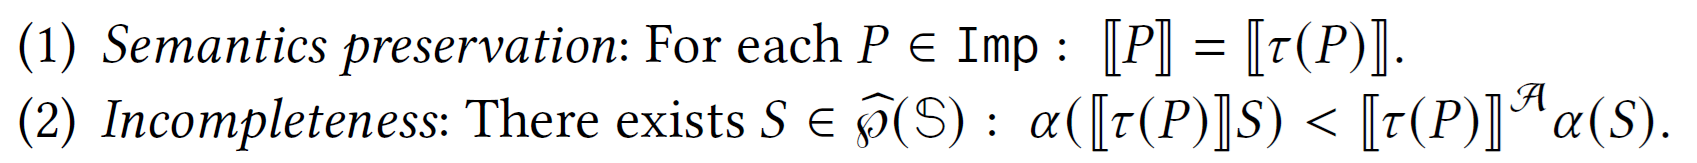
\includegraphics[scale=0.3]{img/목표.png}}

\end{frame}

\begin{frame}
  \frametitle{연구 주제와 비교}
  \uncover<1->{실행 의미는 $\top$이 아니지만, 요약해석 결과는 $\top$이 되는 프로그램 $P$를 만들자(특정 변수 x에 대해서)}
  \begin{align*}
    \uncover<2->{(\llbracket P \rrbracket \mathbb{S})\texttt{x} &\neq \top} \\
    \uncover<2->{(\llbracket P \rrbracket^{\mathcal{A}}\alpha(\mathbb{S}))\texttt{x} &= \top} \\
    \uncover<3->{\alpha(\llbracket P \rrbracket \mathbb{S}) &< \llbracket P \rrbracket^{\mathcal{A}}\alpha(\mathbb{S})}
  \end{align*}

  \uncover<4->{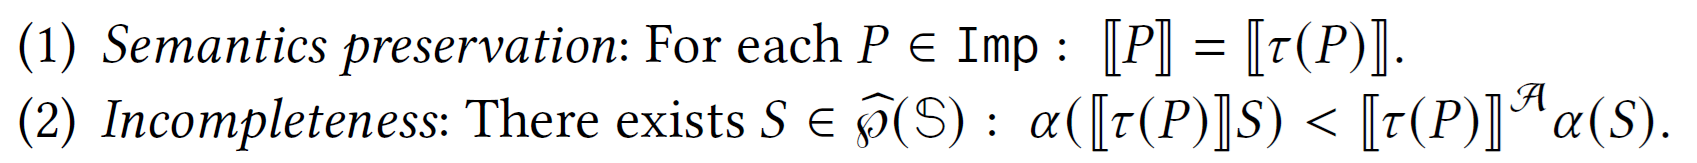
\includegraphics[scale=0.3]{img/목표.png}}
\end{frame}

\section{주요 아이디어}
\begin{frame}[fragile]
  \frametitle{주요 아이디어}
  
  \uncover<1->{요약해석이 제대로 걸러내지 못하는 상태 집합(if문)을 만들자}
  \begin{center}
    \begin{minipage}{0.5\textwidth}
      % uncover 대신 visibleenv 등을 사용하여 환경 전체를 감싸기
      \begin{visibleenv}<2-> 
        \begin{lstlisting}[numbers=left, escapeinside={(*@}{@*)}]
if (*@\textcolor{red}{절대 통과 못하는 조건문}@*)
  (*@이상한 일을 한다@*)
(*@$P$@*)
        \end{lstlisting}
      \end{visibleenv}
    \end{minipage}
  \end{center}

  \hfill

  \uncover<3->{요약해석이 제대로 요약하지 못하는 정수 집합을 만들자}
  \begin{center}
    \begin{minipage}{0.3\textwidth}
      \begin{visibleenv}<4-> 
        \begin{lstlisting}[numbers=left, numberstyle=\small, basicstyle=\small\ttfamily, numbersep=8pt, escapeinside={(*@}{@*)}]
x = (*@\textcolor{red}{1 or 5}@*)
        \end{lstlisting}
      \end{visibleenv}
    \end{minipage}
  \end{center}

\end{frame}



\section{세 가지 방법}


\begin{frame}
  \frametitle{7 REDUCING COMPLETENESS TO INCOMPLETENESS}
  
  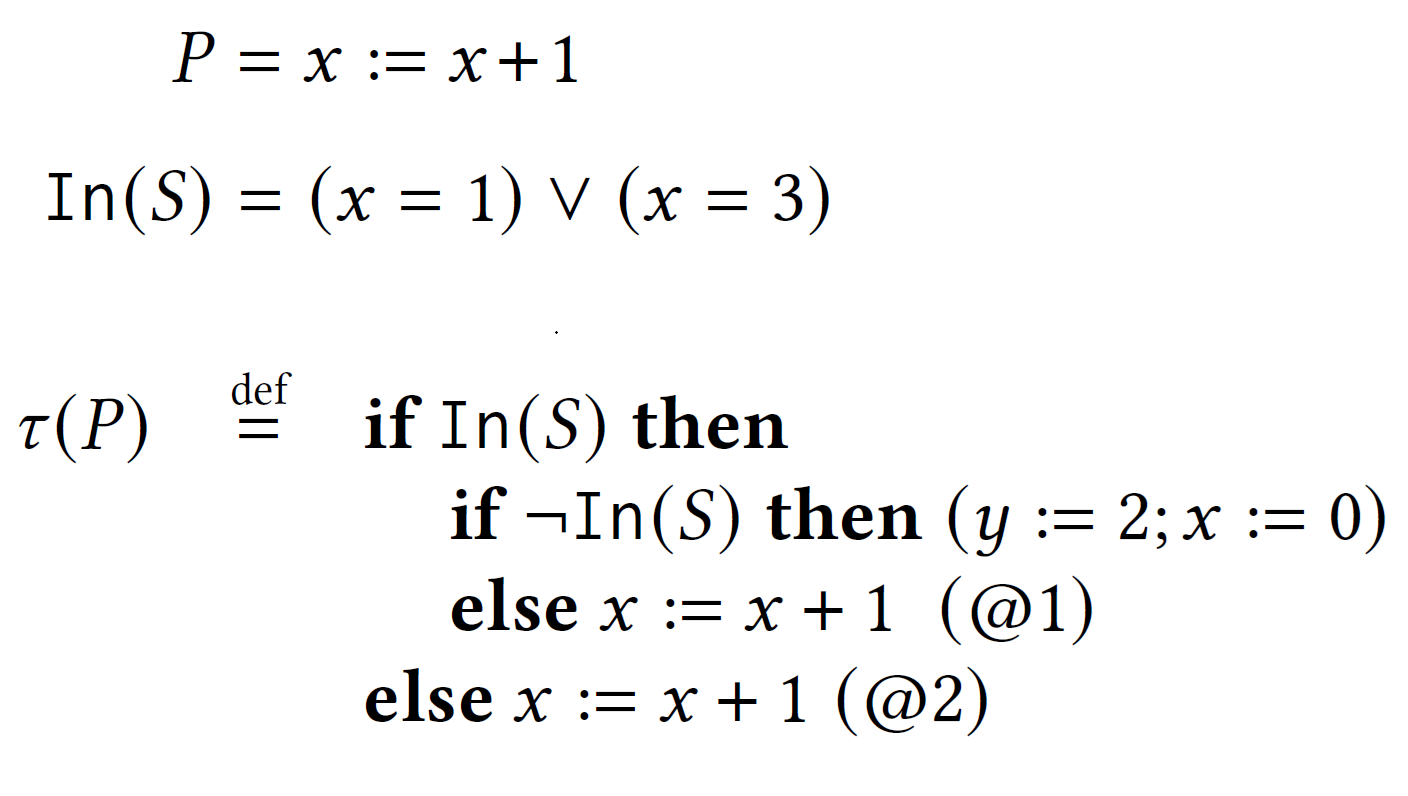
\includegraphics[scale=0.3]{img/7장 예시.png}

  {  
    \large
    \[
    \begin{aligned}
      &\uncover<2->{\llbracket \tau(P) \rrbracket = \llbracket P \rrbracket ?} ~~~~ \uncover<3->{OK!}\\
      &\uncover<4->{\llbracket P \rrbracket^{\mathcal{A}}\alpha(S) < \llbracket \tau(P) \rrbracket^{\mathcal{A}}\alpha(S) ?} ~~~~ \uncover<5-> {OK!}
    \end{aligned}
    \]
  }

\end{frame}


\begin{frame}
  \frametitle{7 REDUCING COMPLETENESS TO INCOMPLETENESS}

  \uncover<1->{
    1. variable finite인 경우

    
\includegraphics[scale=0.15]{img/variable finite.png}
  }

  \uncover<2->{
    2. Rice Theorem의 도움으로,

    
\includegraphics[scale=0.2]{img/rice theorem의 도움.png}
    인 $S$가 존재
  }

  \uncover<3->{
    3. variable finiteness를 이용하여

    
\includegraphics[scale=0.2]{img/m' 찾기.png}
    인 $\mathbb{m}'$이 존재
  }

\end{frame}

\begin{frame}
  \frametitle{7 REDUCING COMPLETENESS TO INCOMPLETENESS}

  
\includegraphics[scale=0.15]{img/variable finite.png}

  
\includegraphics[scale=0.2]{img/rice theorem의 도움.png}

  
\includegraphics[scale=0.2]{img/m' 찾기.png}

  \uncover<2->{
    4. 다음과 같이 프로그램 변환

    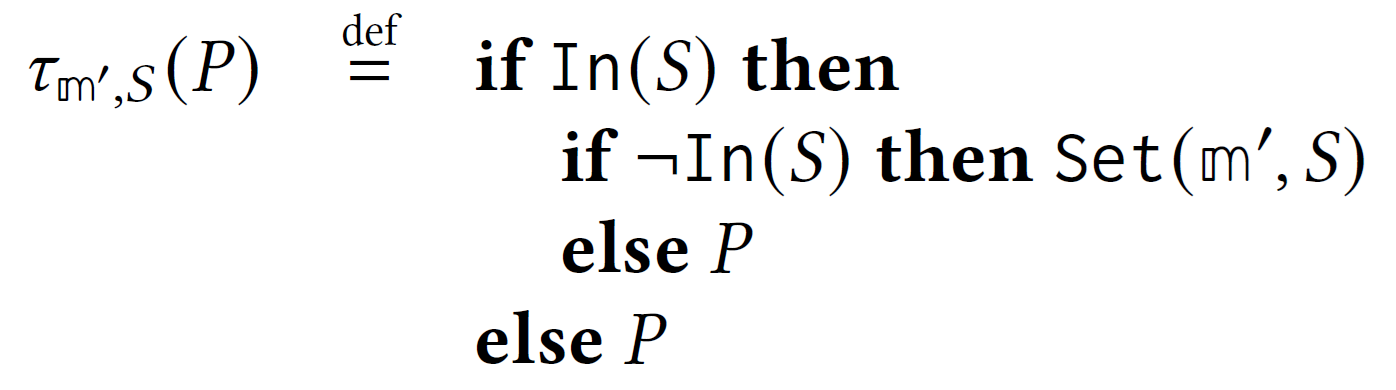
\includegraphics[scale=0.3]{img/7장 아이디어.png}
  }
  \vspace{-12pt}
  {  
    \large
    \[
    \begin{aligned}
      &\uncover<3->{\llbracket \tau(P) \rrbracket = \llbracket P \rrbracket ?} ~~~~ \uncover<4->{OK!}\\
      &\uncover<5->{\llbracket P \rrbracket^{\mathcal{A}}\alpha(S) < \llbracket \tau(P) \rrbracket^{\mathcal{A}}\alpha(S) ?} ~~~~ \uncover<6-> {OK!}
    \end{aligned}
    \]
  }

\end{frame}


\begin{frame}
  \frametitle{8 RICE EXTENSIONALITY OF THE ABSTRACT SEMANTICS}
  \uncover<1->{
    variable finite가 아닌 경우

    
\includegraphics[scale=0.15]{img/not variable finite.png} 인 $S$ 존재
  }
  
  \uncover<2->{
    $x$와 $\mathbb{m}$을 잘 잡아서

    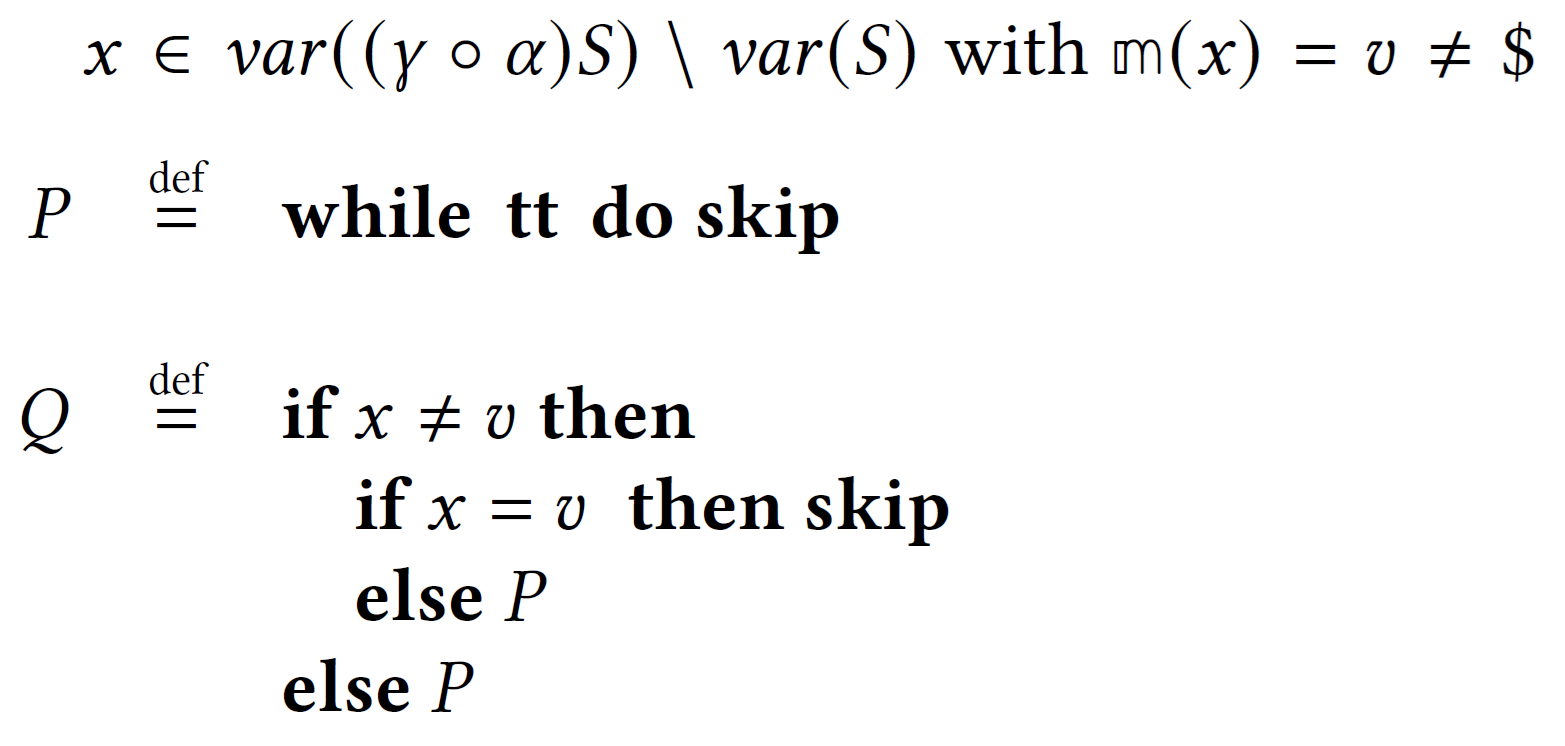
\includegraphics[scale=0.3]{img/8장 아이디어.png}
  }
  
  {  
    \large
    \[
    \begin{aligned}
      &\uncover<3->{\llbracket P \rrbracket = \llbracket Q \rrbracket = \bot} \\
      &\uncover<4->{\llbracket P \rrbracket^{\mathcal{A}} < \llbracket Q \rrbracket^{\mathcal{A}}}
    \end{aligned}
    \]
  }
\end{frame}


\begin{frame}
  \frametitle{8 RICE EXTENSIONALITY OF THE ABSTRACT SEMANTICS}

  
\includegraphics[scale=0.15]{img/not variable finite.png}
  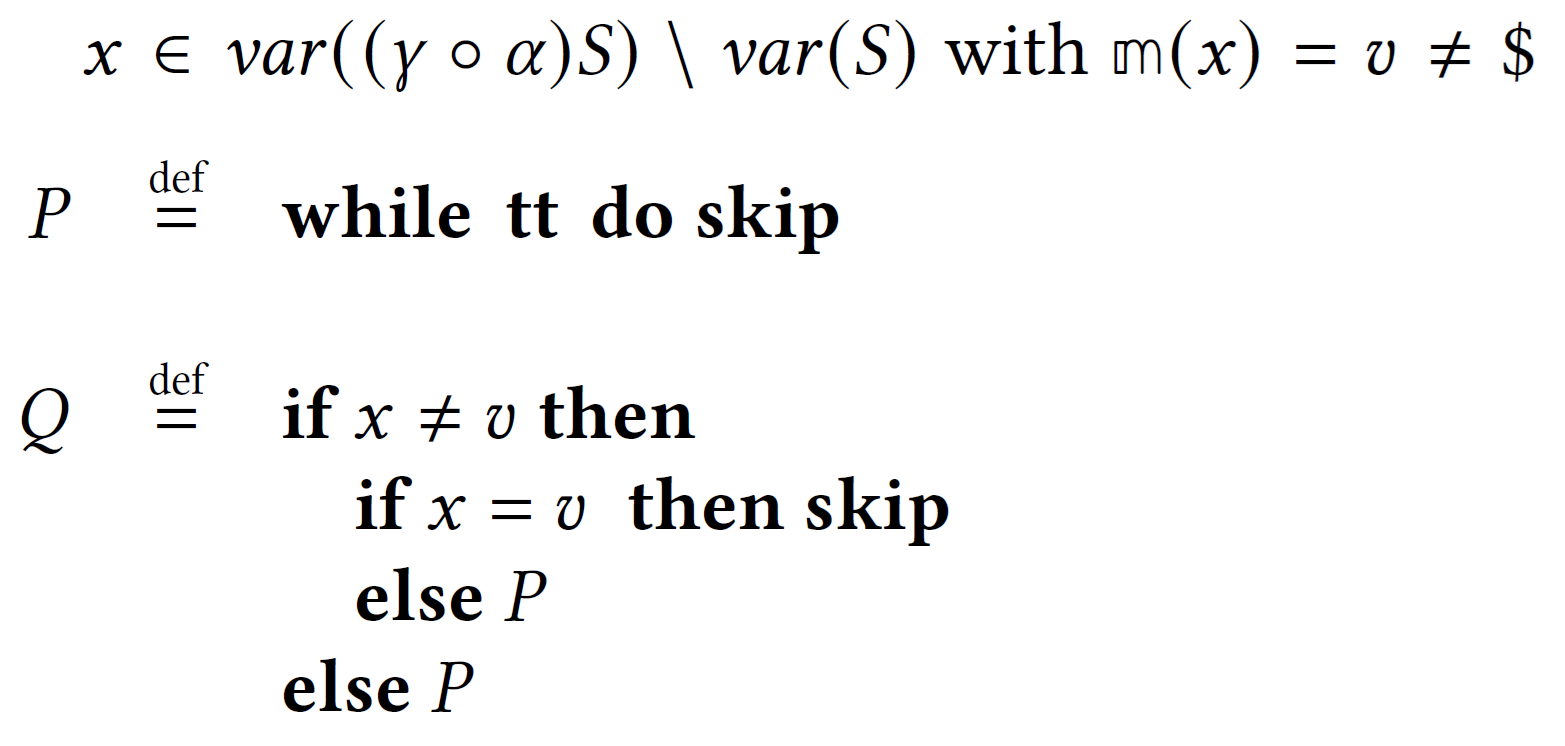
\includegraphics[scale=0.3]{img/8장 아이디어.png}
  
  {  
    \large
    \[
    \begin{aligned}
      &\uncover<2->{\llbracket P \rrbracket = \llbracket Q \rrbracket = \bot} \\
      &\uncover<3->{\llbracket P \rrbracket^{\mathcal{A}} < \llbracket Q \rrbracket^{\mathcal{A}}}
    \end{aligned}
    \]
  }
\end{frame}

\begin{frame}
  \frametitle{9 MAKING ABSTRACTIONS INCOMPLETE BY DATA-FLOW TRANSFORMATIONS}
  
\includegraphics[scale=0.1]{img/9장 아이디어.png}
  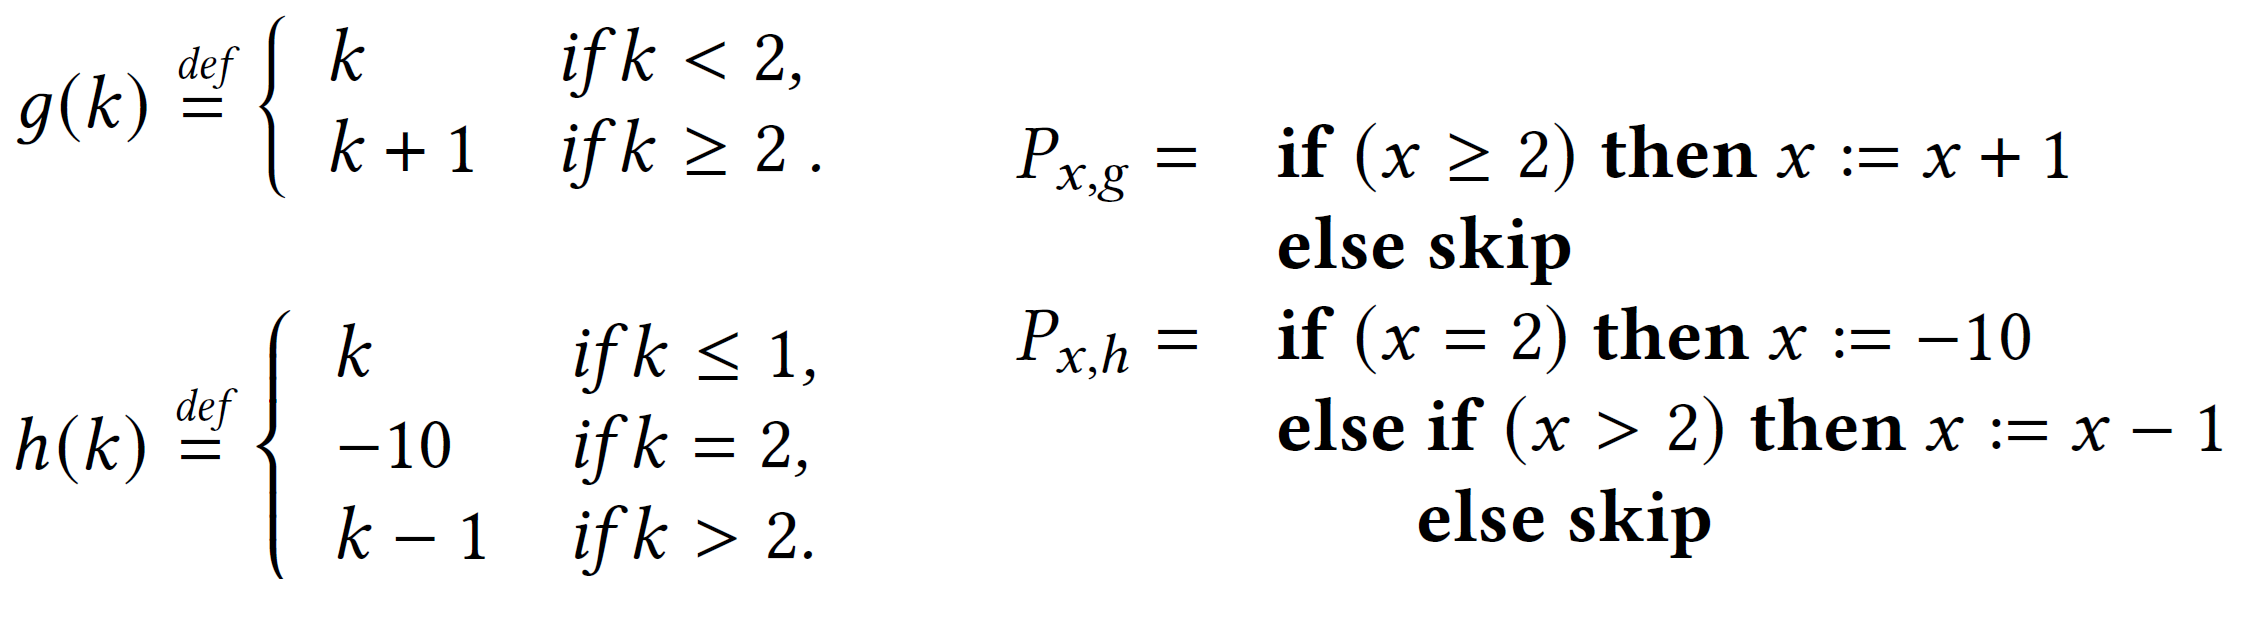
\includegraphics[scale=0.2]{img/9장 예시.png}

  서로 (부분)역함수 관계에 있는 두 함수를 사용해서 요약해석이 제대로 요약하지 못하는 정수 집합으로 다녀오면 됨
  항상 가능한 건 아님
\end{frame}

\section{결론}
\begin{frame}
  \frametitle{결론}
  이런저런 경우에 저런 변환이 항상 존재
  분석기가 제대로 분석하지 못하는 프로그램들의 집합으로도, 기계적인 계산을 다 할 수 있음
\end{frame}


\section{한계점 및 발전 방향}
\begin{frame}
  \frametitle{한계점}
  계속 ``존재성''만 얘기하고, 증명하고 있음
  구체적으로 어떻게 프로그램을 변환하거나 찾는지에 대한 내용이 전혀 없음

  그걸 찾는게 내 목표...인데
  잘 정해진 조건 하에서 불가능을 증명해야 할 수도 있음


  (나) 골탕먹이는 프로그램의 존재성은 rice theorem에서 즉각적으로 나왔는데, 
  (논문) 변환의 존재성은 변환의 기초 구조를 제시한 후 몇 단계를 더 들어가봐야 증명이 가능했음
\end{frame}

\begin{frame}
  \frametitle{발전 방향}
  사실 나도 존재성에만 의지했지, 기계적으로 찾아낼 수 있다는 보장을 가지고 출발한 것이 아님 <- 돌아봐야 할 부분
  이 논문의 아이디어를 응용해서 if문으로 구성된 기본 틀을 주고, 그 안을 합성하게 하는 방법을 생각해 봐야겠음
  if문 말고 while문을 기본 틀로 주는 것도 가능할지도(논문에서는 while문을 제대로 다뤘다고 보기 힘듦)
  while문으로 주면, rice theorem을 직접적으로 사용하기도 하니

  "실제로는 top이 아니다" 를 어떻게 구성하면서 합성해나갈지는 여전히 남아 있는 문제

  다른 난독화 관련 논문들도 뒤져보기
\end{frame}


\end{document}
